\documentclass[a4paper, final]{article}
\usepackage{cmap}
%\usepackage{literat} % Нормальные шрифты
\usepackage[14pt]{extsizes} % для того чтобы задать нестандартный 14-ый размер шрифта
\usepackage[T2A]{fontenc}
\usepackage[UTF8]{inputenc}
\usepackage[russian]{babel}
\usepackage{listings} %листинги
\usepackage{amsmath}
\usepackage{amssymb} % Для красивого значка пустого множества
\usepackage[left=25mm, top=20mm, right=20mm, bottom=20mm, footskip=10mm]{geometry}
\usepackage{ragged2e} %для растягивания по ширине
\usepackage{setspace} %для межстрочного интервала
\usepackage{indentfirst} % для абзацного отступа
\usepackage{moreverb} %для печати в листинге исходного кода программ
\renewcommand\verbatimtabsize{4\relax}
\renewcommand\listingoffset{0.2em} %отступ от номеров строк в листинге
\renewcommand{\arraystretch}{1.4} % изменяю высоту строки в таблице
\usepackage[font=small, singlelinecheck=false, justification=centering, format=plain, labelsep=period]{caption} %для настройки заголовка таблицы
\usepackage{listingsutf8}
\usepackage{xcolor} % цвета
\usepackage{hyperref}% для гиперссылок
\usepackage{enumitem} %для перечислений
\usepackage{titlesec}
\usepackage{graphicx}
\graphicspath{ {./Рисунки/} }
%\usepackage{float}
\usepackage{booktabs}
\usepackage{floatrow}
\usepackage{scalerel} % Stretching images
\usepackage[final]{pdfpages}

\definecolor{apricot}{HTML}{FFF0DA}
\definecolor{mygreen}{rgb}{0,0.6,0}
\definecolor{string}{HTML}{B40000} % цвет строк в коде
\definecolor{comment}{HTML}{008000} % цвет комментариев в коде
\definecolor{keyword}{HTML}{1A00FF} % цвет ключевых слов в коде
\definecolor{morecomment}{HTML}{8000FF} % цвет include и других элементов в коде
\definecolor{captiontext}{HTML}{FFFFFF} % цвет текста заголовка в коде
\definecolor{captionbk}{HTML}{999999} % цвет фона заголовка в коде
\definecolor{bk}{HTML}{FFFFFF} % цвет фона в коде
\definecolor{frame}{HTML}{999999} % цвет рамки в коде
\definecolor{brackets}{HTML}{B40000} % цвет скобок в коде





\AtBeginDocument{\renewcommand{\contentsname}{Содержание}}
\AtBeginDocument{\renewcommand{\refname}{Список источников}}

\floatsetup[table]{style=plain,capposition=bottom}
\setlist[enumerate,itemize]{leftmargin=1.2cm} %отступ в перечислениях

\hypersetup{colorlinks,
  allcolors=[RGB]{010 090 200}} %красивые гиперссылки (не красные)

% подгружаемые языки --- подробнее в документации listings (это всё для листингов)
\lstloadlanguages{ [LaTeX] TeX}
% включаем кириллицу и добавляем кое−какие опции
\lstset{language =[LaTeX] TeX, % выбираем язык по умолчанию
extendedchars=true , % включаем не латиницу
escapechar = | , % |«выпадаем» в LATEX|
frame=tb , % рамка сверху и снизу
commentstyle=\itshape , % шрифт для комментариев
stringstyle =\bfseries} % шрифт для строк

\textheight=24cm % высота текста
\textwidth=16cm % ширина текста
\oddsidemargin=0pt % отступ от левого края
\topmargin=-1.5cm % отступ от верхнего края
\parindent=24pt % абзацный отступ
\parskip=0pt % интервал между абзацами
\tolerance=2000 % терпимость к "жидким" строкам
\flushbottom % выравнивание высоты страниц

\begin{document} % начало документа
\lstset{
  language=SQL, % Язык кода по умолчанию
  morekeywords={*,...}, % если хотите добавить ключевые слова, то добавляйте
  % Цвета
  keywordstyle=\color{keyword}\ttfamily\bfseries,
  %stringstyle=\color{string}\ttfamily,
  stringstyle=\ttfamily\color{red!50!brown},
  commentstyle=\color{comment}\ttfamily,
  morecomment=[l][\color{morecomment}]{\#},
  % Настройки отображения
  breaklines=true, % Перенос длинных строк
  basicstyle=\ttfamily\footnotesize, % Шрифт для отображения кода
  backgroundcolor=\color{bk}, % Цвет фона кода
  frame=single,xleftmargin=\fboxsep,xrightmargin=-\fboxsep, % Рамка, подогнанная к заголовку
  rulecolor=\color{frame}, % Цвет рамки
  tabsize=3, % Размер табуляции в пробелах
  % Настройка отображения номеров строк. Если не нужно, то удалите весь блок
  numbers=left, % Слева отображаются номера строк
  stepnumber=1, % Каждую строку нумеровать
  numbersep=5pt, % Отступ от кода
  numberstyle=\small\color{black}, % Стиль написания номеров строк
  % Для отображения русского языка
  extendedchars=true,
  literate={Ö}{ {\"O} }1
  {~}{ {\textasciitilde} }1
  {а}{ {\selectfont\char224} }1
  {б}{ {\selectfont\char225} }1
  {в}{ {\selectfont\char226} }1
  {г}{ {\selectfont\char227} }1
  {д}{ {\selectfont\char228} }1
  {е}{ {\selectfont\char229} }1
  {ё}{ {\"e} }1
  {ж}{ {\selectfont\char230} }1
  {з}{ {\selectfont\char231} }1
  {и}{ {\selectfont\char232} }1
  {й}{ {\selectfont\char233} }1
  {к}{ {\selectfont\char234} }1
  {л}{ {\selectfont\char235} }1
  {м}{ {\selectfont\char236} }1
  {н}{ {\selectfont\char237} }1
  {о}{ {\selectfont\char238} }1
  {п}{ {\selectfont\char239} }1
  {р}{ {\selectfont\char240} }1
  {с}{ {\selectfont\char241} }1
  {т}{ {\selectfont\char242} }1
  {у}{ {\selectfont\char243} }1
  {ф}{ {\selectfont\char244} }1
  {х}{ {\selectfont\char245} }1
  {ц}{ {\selectfont\char246} }1
  {ч}{ {\selectfont\char247} }1
  {ш}{ {\selectfont\char248} }1
  {щ}{ {\selectfont\char249} }1
  {ъ}{ {\selectfont\char250} }1
  {ы}{ {\selectfont\char251} }1
  {ь}{ {\selectfont\char252} }1
  {э}{ {\selectfont\char253} }1
  {ю}{ {\selectfont\char254} }1
  {я}{ {\selectfont\char255} }1
  {А}{ {\selectfont\char192} }1
  {Б}{ {\selectfont\char193} }1
  {В}{ {\selectfont\char194} }1
  {Г}{ {\selectfont\char195} }1
  {Д}{ {\selectfont\char196} }1
  {Е}{ {\selectfont\char197} }1
  {Ё}{ {\"E} }1
  {Ж}{ {\selectfont\char198} }1
  {З}{ {\selectfont\char199} }1
  {И}{ {\selectfont\char200} }1
  {Й}{ {\selectfont\char201} }1
  {К}{ {\selectfont\char202} }1
  {Л}{ {\selectfont\char203} }1
  {М}{ {\selectfont\char204} }1
  {Н}{ {\selectfont\char205} }1
  {О}{ {\selectfont\char206} }1
  {П}{ {\selectfont\char207} }1
  {Р}{ {\selectfont\char208} }1
  {С}{ {\selectfont\char209} }1
  {Т}{ {\selectfont\char210} }1
  {У}{ {\selectfont\char211} }1
  {Ф}{ {\selectfont\char212} }1
  {Х}{ {\selectfont\char213} }1
  {Ц}{ {\selectfont\char214} }1
  {Ч}{ {\selectfont\char215} }1
  {Ш}{ {\selectfont\char216} }1
  {Щ}{ {\selectfont\char217} }1
  {Ъ}{ {\selectfont\char218} }1
  {Ы}{ {\selectfont\char219} }1
  {Ь}{ {\selectfont\char220} }1
  {Э}{ {\selectfont\char221} }1
  {Ю}{ {\selectfont\char222} }1
  {Я}{ {\selectfont\char223} }1
  {\{}{ { {\color{brackets}\{} } }1 % Цвет скобок {
  {\} }{ { {\color{brackets}\} } } }1 % Цвет скобок }
}

% НАЧАЛО ТИТУЛЬНОГО ЛИСТА
\begin{center}
\hfill \break
\hfill \break
\normalsize{МИНИСТЕРСТВО НАУКИ И ВЫСШЕГО ОБРАЗОВАНИЯ РОССИЙСКОЙ ФЕДЕРАЦИИ\\
 федеральное государственное автономное образовательное учреждение высшего образования «Санкт-Петербургский политехнический университет Петра Великого»\\[10pt]}
\normalsize{Институт компьютерных наук и кибербезопасности}\\[10pt] 
\normalsize{Высшая школа технологий искусственного интеллекта}\\[10pt] 
\normalsize{Направление: 02.03.01 Математика и компьютерные науки}\\

\hfill \break
\hfill \break
\hfill \break
\large{Проектирование WEB приложений}\\
\hfill \break
\large{Отчёт по курсовой работе на тему:}\\
\large{\textbf{«Электронный дневник»\\}}

\hfill \break
\hfill \break
\end{center}
 
\small{ 
\begin{tabular}{lrrl}
\!\!\!Студент, & \hspace{2cm} & & \\
\!\!\!группы 5130201/20102 & \hspace{2cm} & \underline{\hspace{3cm}} & Гаар В.С. \\\\
\!\!\!Преподаватель, \hspace{2cm} & & \\
\!\!\!к.т.н., доц. & \hspace{2cm} & \underline{\hspace{3cm}} &  Попов С.Г. \\\\
&&\hspace{5cm}
\end{tabular}
\begin{flushright}
<<\underline{\hspace{1cm}}>>\underline{\hspace{2.5cm}} 2025 г.
\end{flushright}
}

\hfill \break
\hfill \break
\begin{center} \small{Санкт-Петербург, 2025} \end{center}
\thispagestyle{empty} % выключаем отображение номера для этой страницы

% КОНЕЦ ТИТУЛЬНОГО ЛИСТА
\newpage

\tableofcontents

\newpage

\cleardoublepage
\phantomsection

\addcontentsline{toc}{section}{Введение}
\section*{Введение}
В данном отчете представлено выполнение лабораторной работы по дисциплине <<Проектирование WEB приложений>>. В качестве предметной области был выбран процесс использования электронного дневнивка в школах.
В ходе работы требуется формализовать выбранную предметную область при помощи:
\begin{enumerate}
    \item текстового описания;
    \item ER-диаграмм;
    \item Use case-диаграмм и описаний.
\end{enumerate}

\newpage
\section{Описание предметной области}
Школа как социально-педагогический институт представляет собой структурированную систему, ориентированную на организацию учебно-воспитательного процесса, формирование знаний, навыков и социальных компетенций учащихся. Её функционирование основано на нормативных документах, регламентирующих учебные планы, методы оценивания и взаимодействие между участниками образовательного процесса. Независимо от типа учреждения --- общеобразовательного, профильного или специализированного --- базовый механизм работы включает разделение учащихся на классы по возрастному принципу, закрепление за ними классных руководителей и преподавателей-предметников, а также использование стандартизированных инструментов контроля успеваемости. Учебный год делится на четверти или семестры, в рамках которых осуществляется планирование уроков, проведение контрольных работ, внеклассных мероприятий и итоговой аттестации.

Школьное сообщество включает в себя несколько ключевых групп: учеников, учителей, родителей, администрацию и вспомогательный персонал. Каждая группа играет свою роль в образовательном процессе. Ученики являются основными участниками процесса обучения, они изучают учебные дисциплины, выполняют домашние задания, проходят контрольные работы и экзамены. Учителя обеспечивают подачу материала, разрабатывают учебные программы, оценивают знания учеников и следят за их успеваемостью. Родители осуществляют контроль за обучением своих детей, помогают в подготовке домашних заданий, посещают родительские собрания. Администрация школы управляет учебным процессом, организует расписание, распределяет обязанности среди педагогов и следит за дисциплиной. Вспомогательный персонал включает в себя сотрудников, обеспечивающих функционирование школы: уборщиков, охранников, медицинских работников, бухгалтеров и других специалистов.

% Одной из центральных функций школы является процесс оценивания знаний. Существует несколько типов оценивания: текущие оценки, выставляемые за выполненные задания и ответы на уроках, контрольные и экзаменационные оценки, выставляемые по результатам проверочных работ, итоговые оценки, которые формируются на основе всех предыдущих и определяют уровень усвоения материала за определенный период. В разных системах образования применяются различные системы оценивания: пятибалльная, десятибалльная, буквенная (A, B, C, D, F) и другие. Оценки фиксируются в классном журнале, который ведёт учитель, а также в дневниках, которые заполняют ученики.

Одной из центральных функций школы является процесс оценивания знаний. В школе учителя выставляют ученикам оценки различных типов: текущие (за ответы на уроках и задания), контрольные (по результатам проверочных работ), экзаменационные (за итоговую аттестацию). Эти оценки фиксируются в классном журнале, который ведёт учитель, и дублируются в дневнике, заполняемом учеником. Каждая оценка соответствует одной из принятых систем оценивания: пятибалльной, десятибалльной или буквенной (A-F). Итоговые оценки за учебный период формируются на основе всех полученных баллов, с учётом значимости контрольных и экзаменационных работ.

Основным инструментом фиксации академических результатов является классный журнал --- документ установленного образца, содержащий информацию о посещаемости, темах занятий, домашних заданиях и оценках учащихся. Преподаватели ежедневно вносят в него данные, руководствуясь требованиями к ведению отчётности. Оценки выставляются по шкале, определяемой образовательным стандартом: в младших классах часто применяется система символических отметок (звёздочки, смайлы), в средней и старшей школе --- балльная система. Параллельно с журналом каждый ученик ведёт бумажный дневник, куда записывает задания и текущие оценки, а родители обязаны регулярно его проверять и подтверждать ознакомление подписью. Этот документ служит средством коммуникации между школой и семьёй, однако его эффективность зависит от дисциплины учащегося: пропущенные записи, утрата дневника или неточное отражение информации могут привести к нарушению обратной связи.

Контроль посещаемости осуществляется через отметки о присутствии или отсутствии ученика на уроках, с указанием причин пропусков. Классный руководитель обязан информировать родителей о систематических нарушениях, однако эта процедура требует личных звонков, записей в дневнике или организации встреч, что не всегда позволяет оперативно реагировать на ситуацию. Академическая успеваемость отслеживается через совокупность форм контроля: устные ответы, письменные работы, практические задания и проекты. Итоговые оценки за четверть или полугодие рассчитываются на основе среднего балла, с учётом веса контрольных работ. Преподаватели анализируют результаты для корректировки учебного плана, а администрация формирует сводные отчёты для вышестоящих органов образования.

Домашние задания также являются важной частью учебного процесса. Они позволяют закрепить изученный материал, развить навыки самостоятельного поиска информации и ответственности за выполнение работы в установленные сроки. Домашние задания могут включать в себя письменные работы, подготовку к контрольным, выполнение лабораторных исследований, чтение литературы и другие виды учебной деятельности. Информация о заданных работах традиционно передается ученикам устно на уроках, а также записывается в дневник, что позволяет родителям контролировать учебный процесс.

Помимо учебной деятельности, в школах организуется воспитательная работа. Классные руководители и социальные педагоги следят за социальной адаптацией учеников, проводят воспитательные мероприятия, организуют экскурсии, конкурсы, тематические занятия. Важную роль играют школьные собрания, на которых обсуждаются вопросы дисциплины, успеваемости и организации учебного процесса. Родительские собрания позволяют педагогам и родителям обмениваться информацией, обсуждать проблемы и достижения учеников.

Школьные документы также являются важной частью образовательного процесса. Помимо классного журнала и дневника, используются личные дела учеников, ведомости успеваемости, расписания занятий, приказы администрации, медицинские карты. Эти документы ведутся в бумажном виде и требуют тщательного учета и хранения. Журналы и дневники ежедневно заполняются учителями и учениками, что обеспечивает прозрачность учебного процесса и позволяет отслеживать успеваемость каждого ученика.

Администрация школы обеспечивает хранение журналов в архиве, что позволяет отслеживать динамику успеваемости за несколько лет, однако ручная обработка данных затрудняет оперативный анализ. Формирование отчётов, учёт замен уроков, распределение учебной нагрузки --- эти задачи требуют значительных временных ресурсов из-за зависимости от бумажных носителей.

Организация школьной жизни включает в себя множество аспектов, таких как составление расписания, контроль посещаемости, ведение школьной отчетности, обеспечение безопасности и санитарных норм, организация питания, проведение экзаменационных сессий. Весь этот процесс требует значительных временных затрат со стороны учителей, администрации и других участников образовательного процесса.

С течением времени развитие технологий позволило задуматься о внедрении электронных систем, способных упростить и автоматизировать многие процессы. Основными причинами для создания системы электронного дневника стали:

\begin{enumerate}
  \item \textbf{Упрощение учета успеваемости и посещаемости.} Ведение бумажных журналов требует значительных временных затрат, подвержено человеческим ошибкам, а доступ к информации ограничен. Электронный дневник позволяет в реальном времени вносить оценки и фиксировать посещаемость, обеспечивая моментальный доступ к этим данным.

  \item \textbf{Обеспечение прозрачности и оперативного взаимодействия.} Родители часто сталкиваются с трудностями при получении информации об успехах своих детей. Электронная система позволяет моментально передавать данные об оценках, домашних заданиях, замечаниях учителей, а также отправлять уведомления и сообщения.
  
  \item \textbf{Автоматизация рутинных процессов.} Заполнение дневников, подсчет итоговых оценок, составление отчетности --- все эти задачи могут выполняться автоматически, освобождая время учителей для образовательной деятельности.
  
  \item \textbf{Создание единой базы данных для анализа и прогнозирования.} Электронная система позволяет собирать статистические данные об успеваемости, выявлять проблемные места в учебном процессе, анализировать эффективность методов преподавания и принимать решения на основе объективных данных.
\end{enumerate}


Таким образом, создание системы электронного дневника стало логичным этапом развития школьного образования, направленным на повышение удобства, прозрачности и эффективности учебного процесса.

\subsection{Процессы}
\textbf{Основной процесс: Учет успеваемости и посещаемости}

Этот процесс является основным в образовательном учреждении, поскольку напрямую связан с оцениванием знаний и контролем за посещаемостью. Он включает несколько этапов:
\begin{enumerate}
  \item \textbf{Регистрация посещаемости:} Учитель фиксирует присутствие учеников на занятиях в классном журнале. Это позволяет отслеживать, кто из учеников пропустил уроки, а также предоставляет информацию о нарушениях дисциплины. Посещаемость фиксируется ежедневно, а в конце недели или месяца подводятся итоги.

  \item \textbf{Оценивание успеваемости:} Учителя выставляют оценки за выполнение домашних заданий, ответы на уроках, участие в обсуждениях, контрольные работы, экзамены и другие виды деятельности. Все эти данные фиксируются в классном журнале. В зависимости от системы оценивания (например, пятибалльная, десятибалльная) оценки могут быть получены за различные виды работы.
  
  \item \textbf{Подсчет итоговых оценок:} На основе текущих оценок формируются итоговые, которые показывают уровень знаний ученика за определенный период (например, четверть или год). Эти оценки отражают общую успеваемость ученика и могут использоваться для составления отчетности и принятия решений относительно дальнейшего обучения.
  
  \item \textbf{Доступ к данным:} Родители могут получать информацию о посещаемости и успеваемости своих детей, посещая школу или через школьные собрания. Также, некоторые учителя могут присылать уведомления о пропусках уроков или оценках через письменные записки, которые дети передают родителям.
\end{enumerate}

\textbf{Вспомогательные процессы}
\begin{enumerate}
  \item Передача домашнего задания и обратная связь
  \begin{itemize}
    \item Описание процесса: Учителя обычно озвучивают домашние задания на уроках, записывают их на доске или выдают в письменной форме. Ученики выполняют задания дома, а затем приносят их на следующий урок для проверки. Обратная связь обычно осуществляется устно: учитель комментирует работу ученика на уроке, может поставить отметку или дать рекомендации по улучшению.
  \end{itemize}

  \item Взаимодействие с родителями
  \begin{itemize}
    \item Описание процесса: Родители получают информацию о успехах и проблемах своих детей в процессе учебы через родительские собрания, личные встречи с учителями, а также через письменные уведомления и записки от учителей. В некоторых случаях учителя могут отправлять родителям уведомления через учеников или по телефону, чтобы проинформировать о проблемах с успеваемостью или поведением.
  \end{itemize}

  \item Создание отчетности и статистики
  \begin{itemize}
    \item Описание процесса: Учителя составляют различные отчеты по успеваемости учеников, которые затем передаются администрации школы. Это могут быть отчеты о результатах контрольных работ, итоговых экзаменов, а также об успеваемости класса в целом. Эти данные используются для анализа работы учеников, выработки рекомендаций по улучшению учебного процесса и принятия решений относительно дальнейшего обучения.
  \end{itemize}

  \item Поддержка адаптации учеников с особыми образовательными потребностями
  \begin{itemize}
    \item Описание процесса: В школе могут быть предусмотрены специальные занятия для учеников с особыми образовательными потребностями, такие как индивидуальные занятия с психологом, дополнительная помощь в изучении трудных предметов или адаптированные учебные материалы. Эти ученики получают особое внимание со стороны педагогов и могут получать дополнительные ресурсы для достижения образовательных целей.
  \end{itemize}
  
  \item Организация школьных мероприятий
  \begin{itemize}
    \item Описание процесса: Школа проводит различные мероприятия, такие как экскурсии, спортивные соревнования, конкурсы и другие культурные события. Для их организации составляется расписание, информируются родители, а ученики получают задания, связанные с мероприятием (например, подготовка к конкурсу, участие в театральных постановках или спортивных играх). Учителя и классные руководители координируют эти мероприятия и следят за их успешным проведением.
  \end{itemize}
\end{enumerate}


\newpage
\section{ER-диаграмма}
\subsection{Исходный абзац}
Одной из центральных функций школы является процесс оценивания знаний. В школе учителя выставляют ученикам оценки различных типов: текущие (за ответы на уроках и задания), контрольные (по результатам проверочных работ), экзаменационные (за итоговую аттестацию). Эти оценки фиксируются в классном журнале, который ведёт учитель, и дублируются в дневнике, заполняемом учеником. Каждая оценка соответствует одной из принятых систем оценивания: пятибалльной, десятибалльной или буквенной (A-F). Итоговые оценки за учебный период формируются на основе всех полученных баллов, с учётом значимости контрольных и экзаменационных работ.

\subsection{Изменённый абзац}
Одной из центральных функций школы является оценивание знаний. Оценивание знаний происходит в процессе обучения ученика. Учителя выставляют оценки ученикам. Оценки формируются на основе знаний ученика и могут быть различных типов: текущие (за ответы на уроках и задания), контрольные (по результатам проверочных работ), экзаменационные (за итоговую аттестацию). Эти оценки фиксируются в классном журнале, который ведёт учитель, и дублируются в дневнике, заполняемом учеником. Каждая оценка соответствует одной из принятых систем оценивания: пятибалльной, десятибалльной или буквенной (A-F). Итоговые оценки за учебный период рассчитываются на основе всех ранее полученных оценок.


ER-диаграмма представлена на \hyperlink{diag:er}{рисунке №1}.

\newpage
\hypertarget{diag:er}{}
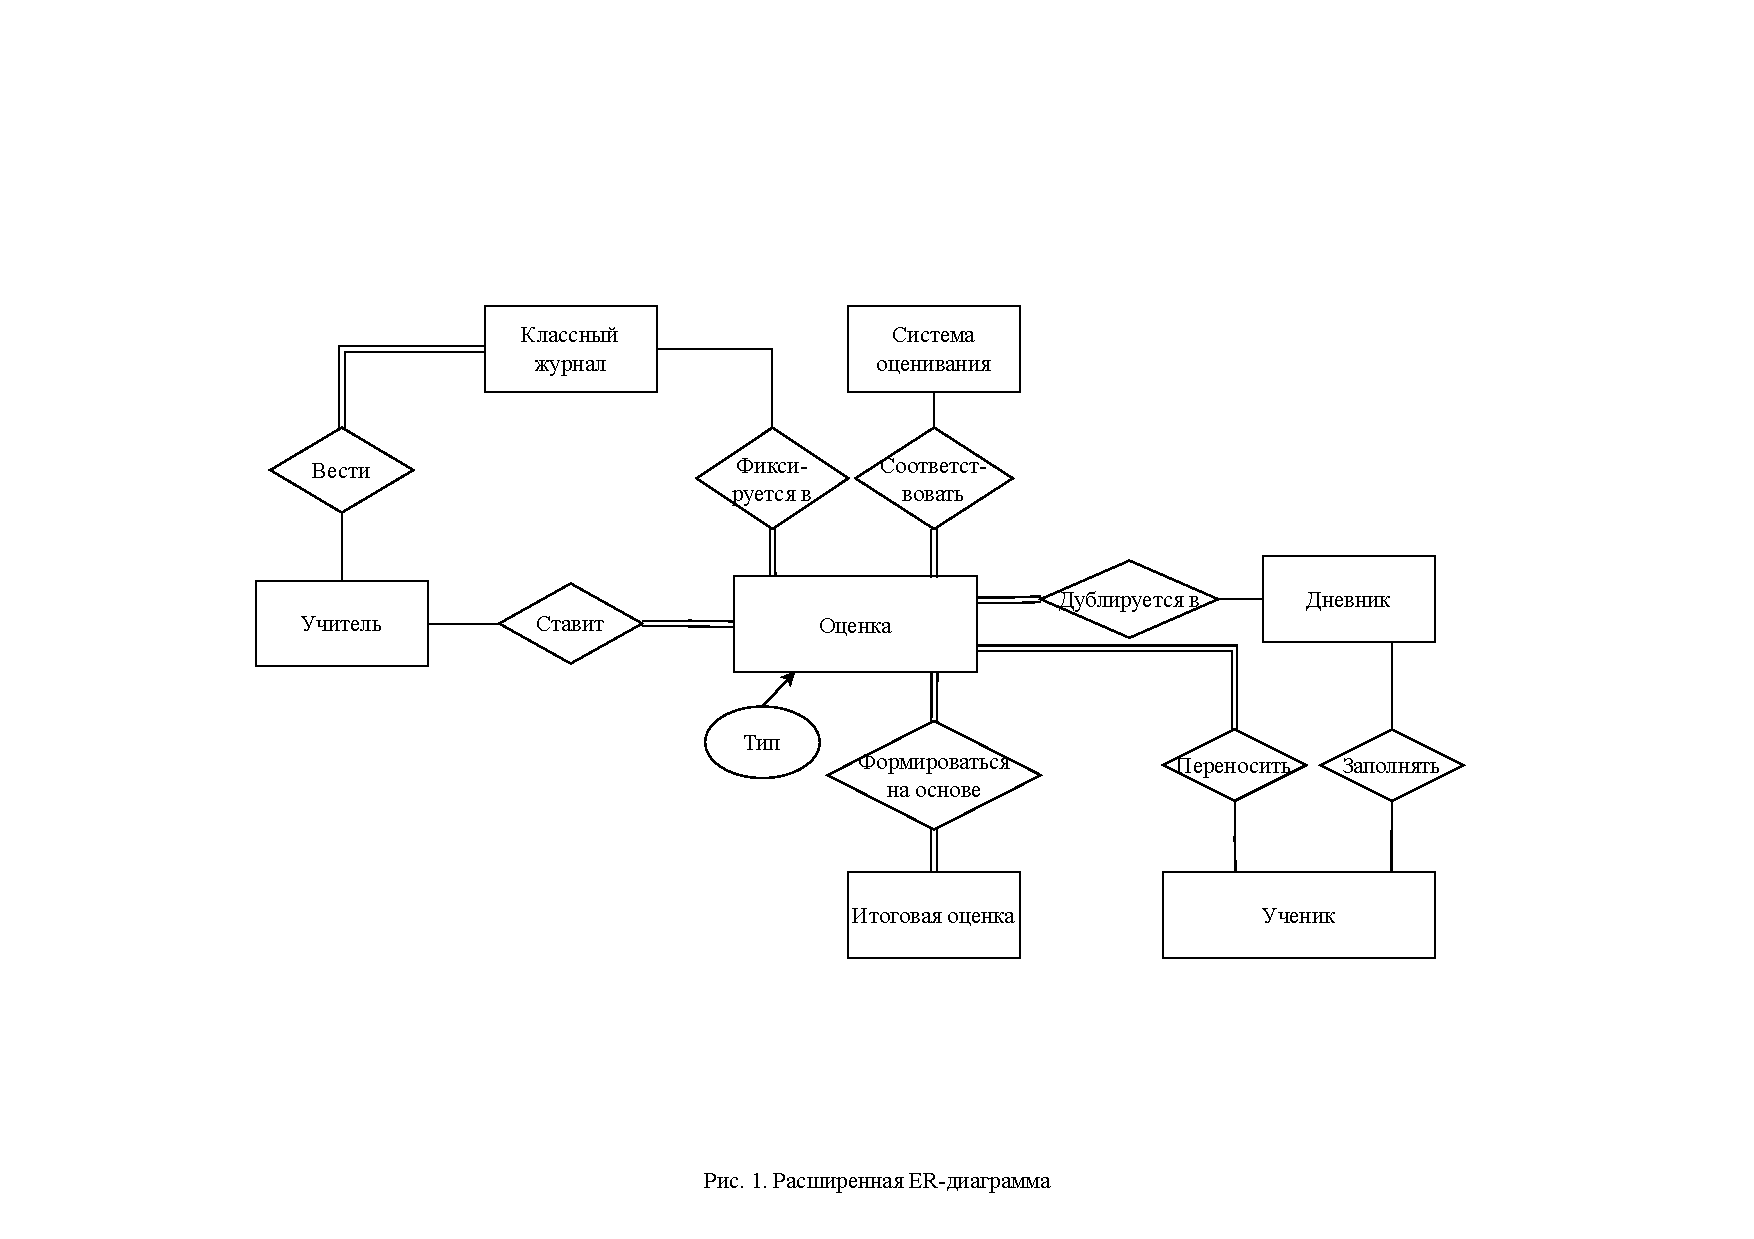
\includepdf[pages=1, fitpaper]{Рисунки/ER.pdf}
\addtocounter{figure}{1}
\newpage

\subsection{Чтение ER-диаграммы}
Школа оценивает знания. Знания оцениваются в процессе обучения ученика. Учителя выставляют оценки ученикам. Оценки формируются на основе знаний ученика и могут быть различных типов: промежуточные, итоговые, экзаменационные. Оценки фиксируются в классном журнале, который ведёт учитель, и дублируются в дневнике, заполняемом учеником. Каждая оценка соответствует одной из систем оценивания с определённой шкалой: пятибалльной, десятибалльной, буквенной (A-F). Некоторые оценки рассчитываются на основе других оценок.

\newpage
\section{Use-cases}
\subsection{1-й уровень}
На Рис.~\ref{img:use_case1} представлена use-case диаграмма первого уровня основного процесса.

\begin{figure}[H]
   \centering
   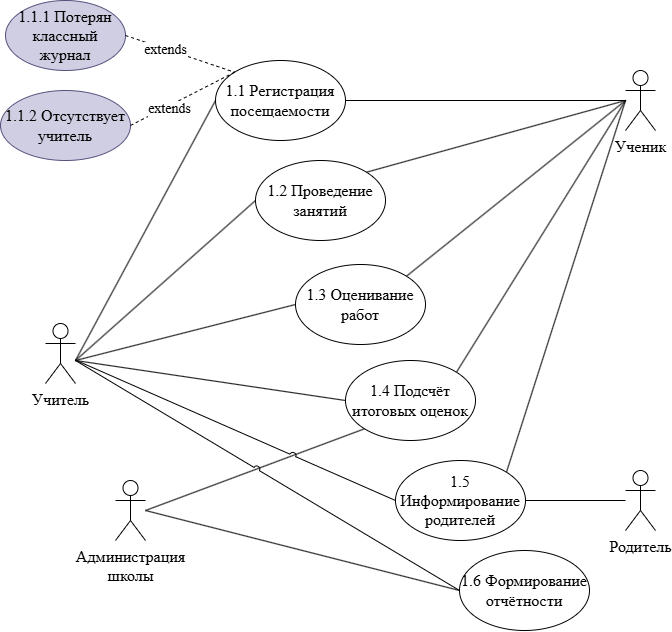
\includegraphics[width=0.7\linewidth]{use_case1.png}
   \caption{Use-case диаграмма основного процесса}
   \label{img:use_case1}
\end{figure}

\begin{enumerate}
  \item Название: Учёт успеваемости и посещаемости.
  \item Акторы: Учитель, Классный руководитель, Ученик, Родитель, Администрация школы.
  \item Входные данные: Классный журнал, дневник ученика, учебный план, расписание уроков.
  \item Триггер: Начало учебного периода.
  \item Выходные данные: Заполненный классный журнал, итоговые оценки за учебный период, отчёты для администрации, подписанный родителем дневник.
\end{enumerate}

\textbf{Основной процесс:}
\begin{enumerate}
  \item [1.1]Регистрация посещаемости.
  \item [1.2]Проведение занятий.
  \item [1.3]Оценивание работ.
  \item [1.4]Подсчет итоговых оценок.
  \item [1.5]Информирование родителей.
  \item [1.6]Формирование отчётности.
\end{enumerate}

\subsection{2-й уровень}
На Рис.~\ref{img:use_case2} представлена use-case диаграмма второго уровня основного процесса.

\begin{figure}[H]
   \centering
   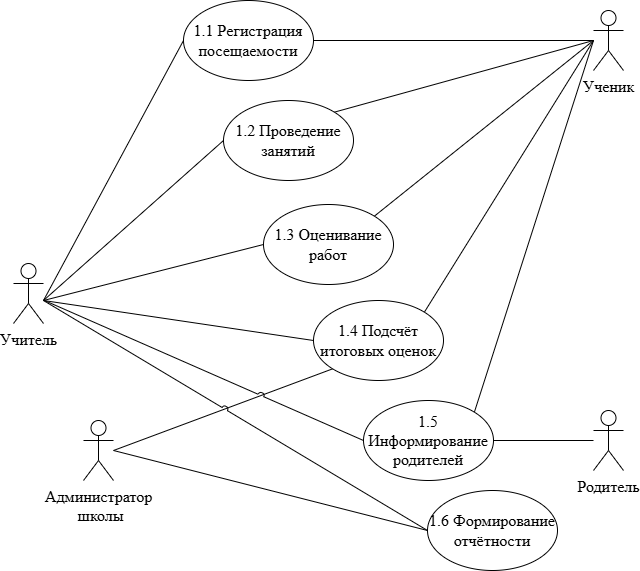
\includegraphics[width=\linewidth]{use_case2.png}
   \caption{Use-case диаграмма второго уровня основного процесса}
   \label{img:use_case2}
\end{figure}

\begin{enumerate}
  \item[1.1] \textbf{Регистрация посещаемости}
  \begin{itemize}
    \item Акторы: Учитель, Ученик.
    \item Входные данные: Список учеников, классный журнал.
    \item Триггер: Начало урока.
    \item Выходные данные: Отметка в классном журнале о присутствии/отсутствии учеников.
  \end{itemize}

  \textbf{Основной процесс:}
  \begin{enumerate}
    \item[1.1.1] Учитель вызывает каждого ученика по списку.
    \item[1.1.2] Ученик подтверждает своё присутствие.
    \item[1.1.3] Учитель отмечает присутствующих и отсутствующих учеников пометками в журнале.
  \end{enumerate}
  
  \textbf{Альтернативные сценарии:}
  \begin{itemize}
    \item[1.1.3.1] Если ученик опоздал, учитель делает отметку <<опоздание>>.
    \item[1.1.3.2] Если ученик пропустил занятие по уважительной причине, учитель отмечает <<уважительная причина>>.
    \item[1.1.3.3] Если ученик пропустил занятие без уважительной причины, учитель отмечает <<неявка>>.
  \end{itemize}
 
  \item[1.2] \textbf{Проведение занятий}
  \begin{itemize}
    \item Акторы: Учитель, Ученик.
    \item Входные данные: Тема урока, учебные материалы.
    \item Триггер: Начало урока согласно расписанию.
    \item Выходные данные: Запись темы и домашнего задания в журнале и дневнике.
  \end{itemize}

  \textbf{Основной процесс:}
  \begin{enumerate}
    \item[1.2.1] Учитель объявляет тему урока и записывает её в журнал.
    \item[1.2.2] Учитель объясняет материал.
    \item[1.2.3] Учитель записывает домашнее задание на доске.
    \item[1.2.4] Ученики переносят задание в дневники.
  \end{enumerate}

  \textbf{Альтернативные сценарии:}
  \begin{itemize}
    \item[1.2.4.1] Ученик не записал задание.
  \end{itemize}

  \item[1.3] \textbf{Оценивание работ}
  \begin{itemize}
    \item Акторы: Учитель, Ученик.
    \item Входные данные: Тетради с домашними заданиями, контрольные работы.
    \item Триггер: Сдача работы учеником.
    \item Выходные данные: Обратная связь ученику, исправление ошибок в работе, оценки в журнале и дневнике.
  \end{itemize}

  \textbf{Основной процесс:}
  \begin{enumerate}
    \item[1.3.1] Ученик сдаёт работу учителю.
    \item[1.3.2] Проверка домашнего задания.
    \item[1.3.3] Ученик переносит оценку в дневник.
  \end{enumerate}

  \textbf{Альтернативные сценарии:}
  \begin{itemize}
    \item[1.3.1.1] Работа не сдана.
    \item[1.3.3.1] Ученик оспаривает оценку.
    \item[1.3.3.2] Работа требует доработки. 
  \end{itemize}

  \item[1.4] \textbf{Подсчёт итоговых оценок}
  \begin{itemize}
    \item Акторы: Учитель, Ученик.
    \item Входные данные: Текущие оценки ученика из классного журнала.
    \item Триггер: Окончание учебного периода (четверть/полугодие).
    \item Выходные данные: Итоговые оценки в классном журнале и дневнике ученика.
  \end{itemize}

  \textbf{Основной процесс:}
  \begin{enumerate}
    \item[1.4.1] Учитель рассчитывает средний балл с учётом контрольных работ.
    \item[1.4.2] Учитель записывает итоговую оценку в журнал.
    \item[1.4.3] Ученик переносит итоговую оценку в дневник.
  \end{enumerate}

  \textbf{Альтернативные сценарии:}
  \begin{itemize}
    \item[1.4.3.1] Ученик оспаривает оценку.
    \item[1.4.3.2] Ученик получает неудовлетворительную итоговую оценку. 
  \end{itemize}

  \item[1.5] \textbf{Информирование родителей}
  \begin{itemize}
    \item Акторы: Учитель, Родитель, Ученик.
    \item Входные данные: Итоговые оценки, замечания.
    \item Триггер: Запрос родителя или окончание учебного периода (четверть/полугодие).
    \item Выходные данные: Подписанный дневник.
  \end{itemize}

  \textbf{Основной процесс:}
  \begin{enumerate}
    \item[1.5.1] Учитель записывает оценки и замечания в дневник.
    \item[1.5.2] Ученик передаёт дневник родителю.
    \item[1.5.3] Родитель проверяет записи и ставит подпись.
  \end{enumerate}

  \textbf{Альтернативные сценарии:}
  \begin{itemize}
    \item[1.5.2.1] Дневник утерян.
    \item[1.5.3.1] Родитель не подписывает дневник из-за разногласий. 
  \end{itemize}
  

  \item[1.6] \textbf{Формирование отчётности}
  \begin{itemize}
    \item Акторы: Учитель, Администрация школы.
    \item Входные данные: Данные из классного журнала.
    \item Триггер: Запрос администрации на отчётность по результатам учебного периода.
    \item Выходные данные: Отчёт о посещаемости и успеваемости класса.
  \end{itemize}

  \textbf{Основной процесс:}
  \begin{enumerate}
    \item[1.6.1] Учитель переносит данные из журнала в отчётную форму.
    \item[1.6.2] Учитель передаёт отчёт завучу.
  \end{enumerate}

  \textbf{Альтернативные сценарии:}
  \begin{itemize}
    \item[1.6.2.1] Отчёт требует исправлений.
  \end{itemize}
\end{enumerate}


\subsection{3-й уровень}
\begin{enumerate}
  \item[1.3.2] \textbf{Проверка домашнего задания}
  \begin{itemize}
    \item Акторы: Учитель, Ученик.
    \item Входные данные: Тетради с домашними заданиями.
    \item Триггер: Сдача домашнего задания учеником.
    \item Выходные данные: Оценка в журнале и дневнике, комментарии к работе.
  \end{itemize}

  \textbf{Основной процесс:}
  \begin{enumerate}
    \item[1.3.2.1] Ученик сдаёт тетрадь с выполненным заданием.
    \item[1.3.2.2] Учитель проверяет работу на соответствие критериям.
    \item[1.3.2.3] Учитель выставляет оценку в журнал и пишет краткий комментарий.
    \item[1.3.2.4] Ученик переносит оценку в дневник и исправляет ошибки по комментариям.
  \end{enumerate}

  \textbf{Альтернативные сценарии:}
  \begin{itemize}
    \item[1.3.2.1.1] Работа не сдана вовремя.
    \item[1.3.2.1.2] Работа списана. 
  \end{itemize}

  \item[1.5.1] \textbf{Запись замечаний в дневник}
  \begin{itemize}
    \item Акторы: Учитель, Ученик.
    \item Входные данные: Замечания о поведении/посещаемости.
    \item Триггер: Нарушение дисциплины или систематические опоздания.
    \item Выходные данные:  Запись в дневнике, подпись родителя.
  \end{itemize}

  \textbf{Основной процесс:}
  \begin{enumerate}
    \item[1.5.1.1] Учитель фиксирует нарушение.
    \item[1.5.1.2] Учитель делает запись в дневнике.
    \item[1.5.1.3] Ученик передаёт дневник родителю.
    \item[1.5.1.4] Родитель ставит подпись, подтверждая ознакомление.
  \end{enumerate} 

  \textbf{Альтернативные сценарии:}
  \begin{itemize}
    \item[1.5.1.3.1] Ученик скрыл замечание.
    \item[1.5.1.4.1] Родитель не согласен с замечанием.
  \end{itemize}

  \item[1.6.1] \textbf{Составление отчёта для администрации}
  \begin{itemize}
    \item Акторы: Учитель.
    \item Входные данные: Данные из классного журнала.
    \item Триггер: Запрос администрации на отчёт.
    \item Выходные данные:  Отчёт об успеваемости класса.
  \end{itemize}

  \textbf{Основной процесс:}
  \begin{enumerate}
    \item[1.6.1.1] Учитель собирает данные из журнала.
    \item[1.6.1.2] Заполняет стандартную форму отчёта.
  \end{enumerate} 

  \textbf{Альтернативные сценарии:}
  \begin{itemize}
    \item[1.6.1.2.1] Несоответствие данных в журнале и отчёте.
  \end{itemize}
\end{enumerate}

\newpage
\section*{Заключение}
\addcontentsline{toc}{section}{Заключение}
Полученные знания могут быть и будут использованы в работе над последующими проектами и заданиями.

\cleardoublepage
\phantomsection
\newpage
%Список источников
\begin{thebibliography}{0}
	% \bibitem{bib:mysqldoc}
	% MySQL Documentation [Электронный ресурс] URL: https://dev.mysql.com/doc/ (дата обращения 30.04.2024).
\end{thebibliography}
\addcontentsline{toc}{section}{Список источников}
\end{document}